\documentclass[11pt]{article}


\usepackage{geometry}
\usepackage{subcaption} 
\geometry{letterpaper}


\usepackage{doc}
\usepackage{cite}
\usepackage[margin=1cm]{caption}

\usepackage{url}


\usepackage{graphicx}
\usepackage{epstopdf}
\DeclareGraphicsRule{.tif}{png}{.png}{`convert #1 `dirname #1`/`basename #1 .tif`.png}


\title{A ``Dream'' Interface Design}
\author{Rachel Rivera}
\date{November 25, 2014}


\begin{document}


\maketitle


\begin{abstract}
This investigation presents a ``dream'' user interface design for touchscreen mobile devices. This design aims to tackle the touchscreen usability issue of insufficient feedback as well as provide an interface that is user-friendly for individuals with visual impairments and individuals without visual impairments alike. Of the five prevalent usability metrics within the field of Interaction Design, the three metrics of learnability, efficiency, and errors were particularly significant in the creation and development of this interface design \cite{Nielsen:1993:UE:529793}.
\end{abstract}


\pagebreak
\tableofcontents



\pagebreak


\section{Introduction}
\label{Introduction}

Mobile devices are ubiquitous in contemporary society. The latest figures from the United Nations' telecommunications agency estimate that there are around 6.8 billion cell-phone subscriptions in the world \cite{UNTelecommunications	}. Thus, the investigation and development of usable interfaces for mobile devices is a significant research topic.

Many mobile devices today utilize touchscreens instead of physical keyboards or buttons. This allows for a larger display without increasing the size of the device. Furthermore, touchscreen keyboards and buttons have the ability to change their layout based on user input and disappear when not needed. To compensate for the lack of tactile feedback provided by physical keys and buttons, touchscreen devices often include aural feedback in the form of audible clicks from a speaker. Haptic feedback in the form of device vibrations is often included as well.

Although these alternative aural and haptic signals are provided for the user, the literature suggests that overall feedback is still insufficient and remains a major usability issue with touchscreen devices. \cite{Tinwala:2010:ETE:18	68914.1868972, Kane:2011:UGB:1978942.1979001, Hardy:2008:TIT:1409240.1409267, El-Glaly:2013:TTF:2460625.2460665, Buxton:1986:HID:22339.22386}. A study by Hussain Tinwala and Scott MacKenzie submits that the lack of tactile feedback requires heightened visual attention from the user, which diverts the user's concentration from the thoughts being expressed \cite{Tinwala:2010:ETE:18 68914.1868972}. The lack of tactile feedback not only diverts the attention of some users, but it also makes the device  almost entirely unusable for other users. A study from Virginia Polytechnic Institute and State University demonstrates how touchscreen mobile devices do not provide sufficient feedback for Individuals with Blindness or Severe Visual Impairment (IBSVI). These users are only able to develop a spatial mental model for the touchscreen through ``dead reckoning'' \cite{El-Glaly:2013:TTF:2460625.2460665}. 

Thus, the aim of this investigation is to propose a ``dream'' interface design that addresses the usability issue of insufficient feedback.


\section{System Description}
\label{System Description}

In this investigation, I present a ``dream'' interface design for touchscreen mobile devices that focuses on providing the user with as much as feedback as possible. This feedback is designed in a way that aims to be helpful for users with visual impairments and users without visual impairments alike. The design in its entirety was created with the usability metrics of learnability, efficiency, and error rate in mind.

This ``dream'' interface design incorporates functionality of a product that is currently being developed by Tactus Technology \cite{Tactus}. Tactus Technology, a company based in Fremont, California, creates technology that can reshape the surface of touchscreens on demand. The technology allows real physical buttons to dynamically appear and disappear into a flat touchscreen (see Figure~\ref{tactus1}). Small fluid channels are routed throughout the Tactile Layer and enable fluid to expand the top polymer layer to create the physical buttons \cite{Tactus}.

Although this technology from Tactus is extremely bleeding-edge, the prototypes have already received a fair amount of recognition \cite{CNN, I-Zone, PCMag, Wired}. Reviewers have articulated how the technology seems to be ``downright magical'' \cite{CNN}. Though the look and feel of Tatctus technology seems totally futuristic, the technology is already beginning to appear in consumer devices. In 2013, Touch Revolution, the largest-volume glass projected capacitive multi-touch screen manufacturer in the world, announced a partnership with Tactus Technology \cite{TactusAvailability}. The technologies from the two companies are being combined and manufactured into consumer devices today \cite{TactusAvailability}. Not only is this technology becoming more  available, but it is becoming more customizable as well. Companies will soon be able to customize the panel for different types of buttons, say for example, the buttons on a TV remote \cite{CNN}.

\begin{figure}[ht]
\centering
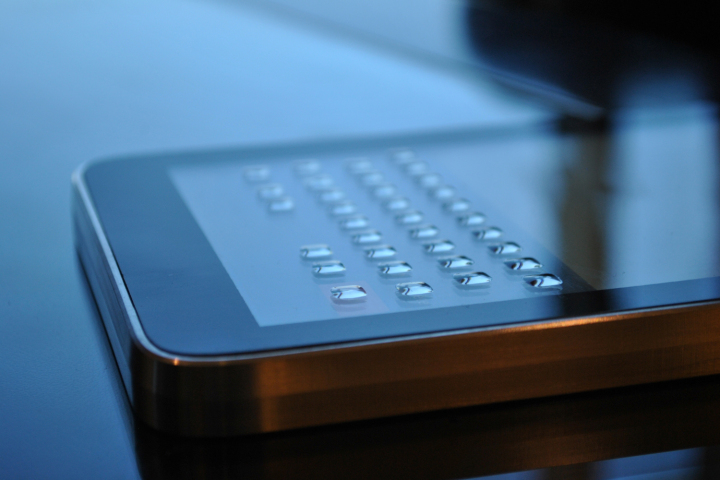
\includegraphics[width=4.5in]{tactus2.jpg} 
\caption{Tactus Technology keyboard}
\label{tactus1}
\end{figure}

This ``dream'' user interface design makes use of the varied tactile feedback that the technology from Tactus can provide.


\section{Top-Level Design}
The objective of this ``dream'' interface design is to make mobile touchscreen devices more usable for individuals with visual impairments and individuals without visual impairments alike. The three main features of this design are the optional physical grid, the ``intelligent'' tactile buttons, and the aural feedback. 


\subsection{Optional Physical Grid}
The design incorporates Tactus technology in order to provide an optional tactile grid for the device (see Figure~\ref{wireframe-grid}). The grid layout would consist of a set of very thin, three-dimensional horizontal and vertical lines. If the grid is enabled by the user, the set of horizontal and vertical lines appears on the screen. If the grid is disabled by the user, the lines recede. The horizontal and vertical lines are arranged with equal space between each line. The main purpose of this grid is to help IBSVI formulate a mental reference for location awareness. The fact that the grid can easily be disabled makes this feature unobtrusive for users who do not find benefit from it.


\begin{figure}[ht]
\centering
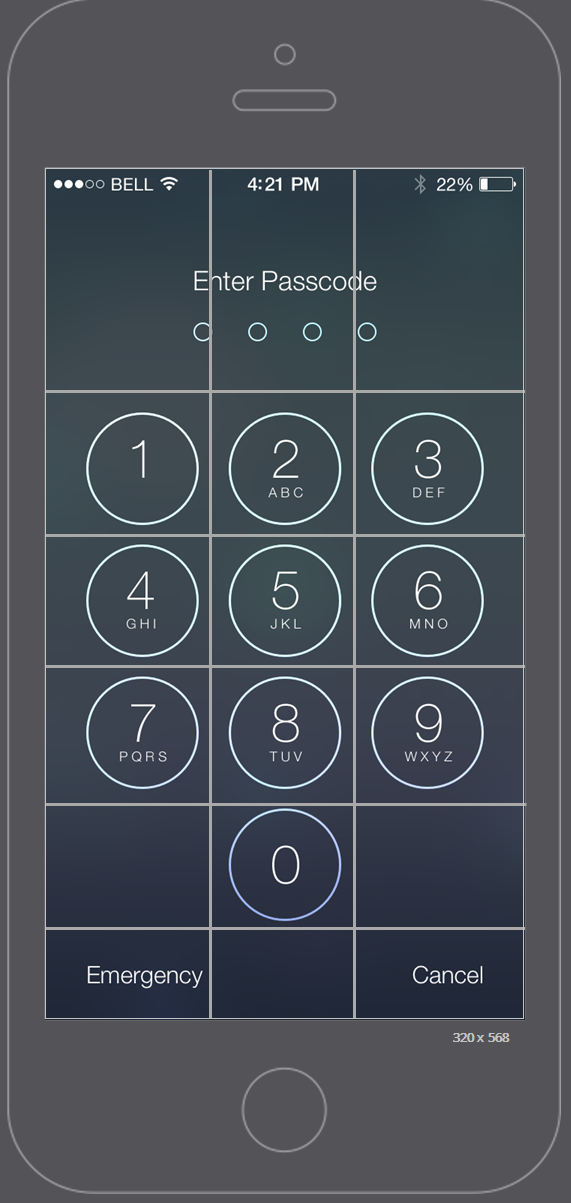
\includegraphics[width=2in]{wireframe-grid.png} 
\caption{A simple wireframe demonstrating the concept of the grid layout. Each line in the figure would actually be a physical line that appears on the device's screen with the use of Tactus' microfluidic technology.}
\label{wireframe-grid}
\end{figure}

\subsection{``Intelligent'' Tactile Buttons}
The interface design also includes tactile buttons that utilize Tactus' microfluidic technology in order to rise up and recede in an ``intelligent'' manner (see Figure~\ref{buttons}). Ideally, only buttons applicable to the input of the user or current state of the device would appear at any given time. For example, in an instance where the user is provided with a binary yes/no choice, only two tactile buttons should appear---one for yes and one for no. Similarly, if all possible buttons were applicable for a given situation, then all possible buttons should appear.

\begin{figure}[ht]
\centering
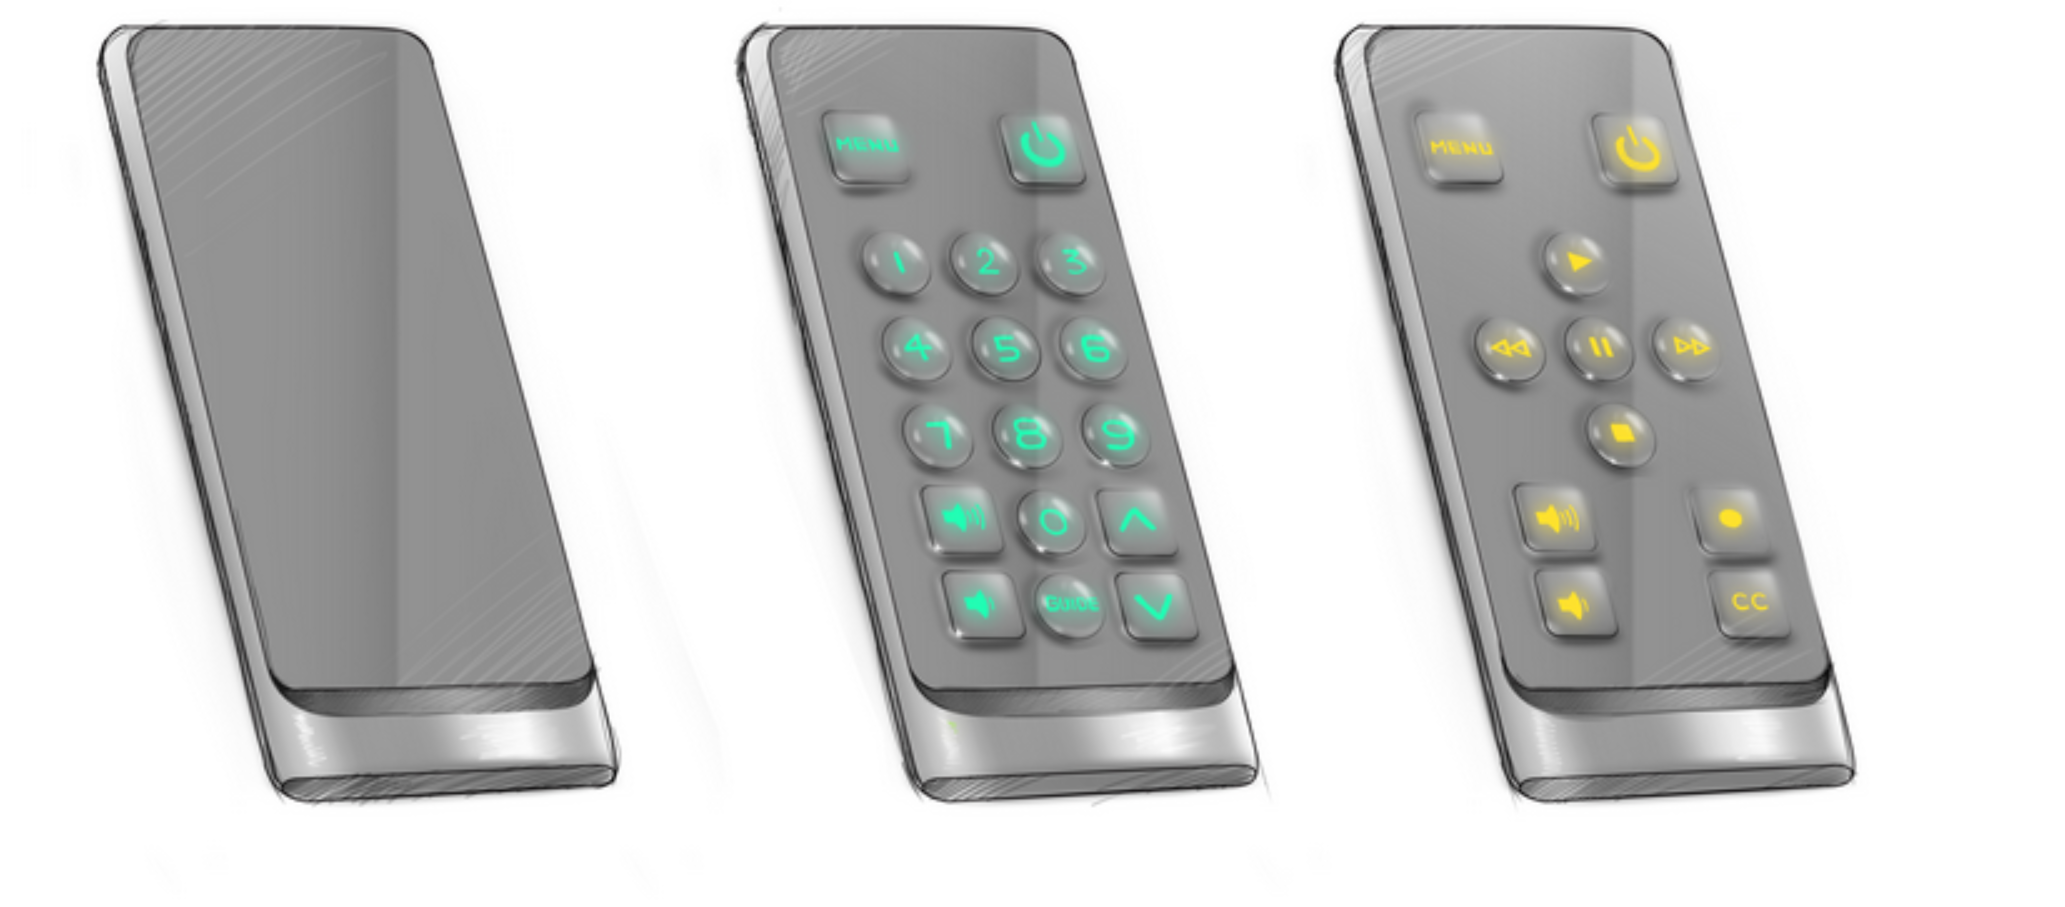
\includegraphics[width=6in]{buttons.png}
\caption{A simple representation demonstrating the idea of different subsets of buttons rising up on the same surface at different times.}
\label{buttons}
\end{figure}

\subsection{Aural Feedback}
\label{aural-feedback}
The design of this interface was created in such a way that the tactile aspects can operate in conjunction with other technologies that provide aural feedback. Since the grid and tactile buttons can only help the user know \textit{where} an application is, this aural feedback can inform the user of exactly \textit{what} an application is.

This type of feedback should not be too difficult to implement as there already exists technology that provides similar aural feedback. For example, the Apple operating system, iOS, has the VoiceOver screen reader that provides a spoken description of everything happening on the screen \cite{VoiceOver}. The Android OS has a similar service called TalkBack, which adds spoken and audible feedback to the device \cite{TalkBack}.


\section{Usage Scenarios}
There exist several usage scenarios for this interface design. One such scenario is when an Individual with Blindness of Severe Visual Impairment (IBSVI) attempts to locate an application on a touchscreen mobile device. Sighted users employ vision to figure out what and where to touch. Since IBSVI cannot do this, typical touchscreen devices lack accessibility for IBSVI. As previously touched on in Section~\ref{aural-feedback}, a typical solution to this problem is to use voice over technology to provide information about what is on the screen at any given time. However, there is nothing to guide IBSVI to the location of a specific application in the first place. Since there are no landmarks to support navigation for the IBSVI, the user must use dead-reckoning and trial-and-error methods in order to find applications specified by the voice over technology. 

The design of this interface addresses this problem as the tactile grid and the three-dimensional buttons provide additional landmarks for IBSVI. These landmarks aim to allow IBSVI interact more efficiently and effectively with the touch device and its voice over functionality. Ideally, the voice over functionality would be able to tell the user the exact cell in the grid in which the desired application is located. The user could then find the application much more easily.

Another use case for this interface is when some functionality of an application is disabled. Say, for example, that a user cannot take any more photos on their mobile device because they are out of memory. Some ``intelligent'' tactile picture-taking button could recede when this happens to communicate to the user that photo taking functionality is disabled. More generally, the``intelligent'' tactile buttons can be useful in indicating to the user what choices they have at any given time.

\section{Rationale}
The driving force behind the creation and development of this interface design is feedback. Feedback is considered a critical concept in the field of interaction design. Donald Norman, the author of \textit{The Design of Everyday Things}, repeatedly articulates the importance of showing the effect of an action \cite{Norman02}. Without feedback, the user is always wondering whether or not anything has happened. In this ``dream'' interface design, the tactile feedback from the physical buttons serves to help the user understand when an action has been performed. Furthermore, the additional aural feedback of the design also assists in communicating the current state of the device to the user.

Another interaction design concept that Norman discusses is how systems with more options and less feedback can be very difficult to use \cite{Norman02}. My design includes ``intelligent'' physical buttons so that the device provides the user with the minimum number of options any given time. Since the buttons will only appear in situations when they are needed, it narrows the options for the user. This ultimately decreases the cognitive load on the user as they have less buttons from which to choose.

This design was also created in a way that allows IBSVI to engage their spatial cognition, perception and sensing resources while interacting with touchscreen mobile devices. A previous study from Virginia Polytechnic Institute and State University demonstrates how touchscreen devices with some kind of a physical overlay typically improve learnability and efficiency while decreasing error rates for IBSVI \cite{El-Glaly:2013:TTF:2460625.2460665}. The optional grid of this ``dream'' interface is very similar to the physical overlay from the study, and should thus improve usability metrics for IBSVI with touchscreen phones.


\section{Usability Metric ``Forecast''}
If implemented then tested, I would expect this interface to have better usability metrics with respect to learnability than conventional touchscreen mobile devices.  More physical landmarks allow all users to engage their spatial cognition more fully when interacting with touchscreens. Furthermore, evidence in the past has demonstrated  that more tactile feedback can make a system more learnable \cite{El-Glaly:2013:TTF:2460625.2460665, conf/chi/KaneWL11}. 

Studies in the past have also suggested that more tactile feedback makes IBSVI more efficient when using the system \cite{El-Glaly:2013:TTF:2460625.2460665, Buxton:1986:HID:22339.22386}. This interface might, however, be slightly less efficient for users who do not have visual impairments. These users will have to lift their fingers more and press down significantly harder with the tactile buttons. I would expect this difference in efficiency to be negligible though.

I would also expect all users to be more perform less errors as well as be more satisfied with this ``dream'' interface. As tactile buttons are harder to press, there would be less likelihood that one would be pressed accidentally. Furthermore, studies have shown that most users enjoy tactile feedback \cite{Freeman:2014:TFA:2663204.2663280}.

\clearpage


\bibliography{mybib}{}
\bibliographystyle{plain}
\end{document}

\end{document}
	